% Options for packages loaded elsewhere
\PassOptionsToPackage{unicode}{hyperref}
\PassOptionsToPackage{hyphens}{url}
\PassOptionsToPackage{dvipsnames,svgnames,x11names}{xcolor}
%
\documentclass[
  11pt,
  letterpaper,
  DIV=11,
  numbers=noendperiod]{scrartcl}

\usepackage{amsmath,amssymb}
\usepackage{iftex}
\ifPDFTeX
  \usepackage[T1]{fontenc}
  \usepackage[utf8]{inputenc}
  \usepackage{textcomp} % provide euro and other symbols
\else % if luatex or xetex
  \usepackage{unicode-math}
  \defaultfontfeatures{Scale=MatchLowercase}
  \defaultfontfeatures[\rmfamily]{Ligatures=TeX,Scale=1}
\fi
\usepackage{lmodern}
\ifPDFTeX\else  
    % xetex/luatex font selection
\fi
% Use upquote if available, for straight quotes in verbatim environments
\IfFileExists{upquote.sty}{\usepackage{upquote}}{}
\IfFileExists{microtype.sty}{% use microtype if available
  \usepackage[]{microtype}
  \UseMicrotypeSet[protrusion]{basicmath} % disable protrusion for tt fonts
}{}
\makeatletter
\@ifundefined{KOMAClassName}{% if non-KOMA class
  \IfFileExists{parskip.sty}{%
    \usepackage{parskip}
  }{% else
    \setlength{\parindent}{0pt}
    \setlength{\parskip}{6pt plus 2pt minus 1pt}}
}{% if KOMA class
  \KOMAoptions{parskip=half}}
\makeatother
\usepackage{xcolor}
\setlength{\emergencystretch}{3em} % prevent overfull lines
\setcounter{secnumdepth}{-\maxdimen} % remove section numbering
% Make \paragraph and \subparagraph free-standing
\makeatletter
\ifx\paragraph\undefined\else
  \let\oldparagraph\paragraph
  \renewcommand{\paragraph}{
    \@ifstar
      \xxxParagraphStar
      \xxxParagraphNoStar
  }
  \newcommand{\xxxParagraphStar}[1]{\oldparagraph*{#1}\mbox{}}
  \newcommand{\xxxParagraphNoStar}[1]{\oldparagraph{#1}\mbox{}}
\fi
\ifx\subparagraph\undefined\else
  \let\oldsubparagraph\subparagraph
  \renewcommand{\subparagraph}{
    \@ifstar
      \xxxSubParagraphStar
      \xxxSubParagraphNoStar
  }
  \newcommand{\xxxSubParagraphStar}[1]{\oldsubparagraph*{#1}\mbox{}}
  \newcommand{\xxxSubParagraphNoStar}[1]{\oldsubparagraph{#1}\mbox{}}
\fi
\makeatother

\usepackage{color}
\usepackage{fancyvrb}
\newcommand{\VerbBar}{|}
\newcommand{\VERB}{\Verb[commandchars=\\\{\}]}
\DefineVerbatimEnvironment{Highlighting}{Verbatim}{commandchars=\\\{\}}
% Add ',fontsize=\small' for more characters per line
\usepackage{framed}
\definecolor{shadecolor}{RGB}{35,38,41}
\newenvironment{Shaded}{\begin{snugshade}}{\end{snugshade}}
\newcommand{\AlertTok}[1]{\textcolor[rgb]{0.58,0.85,0.30}{\textbf{\colorbox[rgb]{0.30,0.12,0.14}{#1}}}}
\newcommand{\AnnotationTok}[1]{\textcolor[rgb]{0.25,0.50,0.35}{#1}}
\newcommand{\AttributeTok}[1]{\textcolor[rgb]{0.16,0.50,0.73}{#1}}
\newcommand{\BaseNTok}[1]{\textcolor[rgb]{0.96,0.45,0.00}{#1}}
\newcommand{\BuiltInTok}[1]{\textcolor[rgb]{0.50,0.55,0.55}{#1}}
\newcommand{\CharTok}[1]{\textcolor[rgb]{0.24,0.68,0.91}{#1}}
\newcommand{\CommentTok}[1]{\textcolor[rgb]{0.48,0.49,0.49}{#1}}
\newcommand{\CommentVarTok}[1]{\textcolor[rgb]{0.50,0.55,0.55}{#1}}
\newcommand{\ConstantTok}[1]{\textcolor[rgb]{0.15,0.68,0.68}{\textbf{#1}}}
\newcommand{\ControlFlowTok}[1]{\textcolor[rgb]{0.99,0.74,0.29}{\textbf{#1}}}
\newcommand{\DataTypeTok}[1]{\textcolor[rgb]{0.16,0.50,0.73}{#1}}
\newcommand{\DecValTok}[1]{\textcolor[rgb]{0.96,0.45,0.00}{#1}}
\newcommand{\DocumentationTok}[1]{\textcolor[rgb]{0.64,0.20,0.25}{#1}}
\newcommand{\ErrorTok}[1]{\textcolor[rgb]{0.85,0.27,0.33}{\underline{#1}}}
\newcommand{\ExtensionTok}[1]{\textcolor[rgb]{0.00,0.60,1.00}{\textbf{#1}}}
\newcommand{\FloatTok}[1]{\textcolor[rgb]{0.96,0.45,0.00}{#1}}
\newcommand{\FunctionTok}[1]{\textcolor[rgb]{0.56,0.27,0.68}{#1}}
\newcommand{\ImportTok}[1]{\textcolor[rgb]{0.15,0.68,0.38}{#1}}
\newcommand{\InformationTok}[1]{\textcolor[rgb]{0.77,0.36,0.00}{#1}}
\newcommand{\KeywordTok}[1]{\textcolor[rgb]{0.81,0.81,0.76}{\textbf{#1}}}
\newcommand{\NormalTok}[1]{\textcolor[rgb]{0.81,0.81,0.76}{#1}}
\newcommand{\OperatorTok}[1]{\textcolor[rgb]{0.81,0.81,0.76}{#1}}
\newcommand{\OtherTok}[1]{\textcolor[rgb]{0.15,0.68,0.38}{#1}}
\newcommand{\PreprocessorTok}[1]{\textcolor[rgb]{0.15,0.68,0.38}{#1}}
\newcommand{\RegionMarkerTok}[1]{\textcolor[rgb]{0.16,0.50,0.73}{\colorbox[rgb]{0.08,0.19,0.26}{#1}}}
\newcommand{\SpecialCharTok}[1]{\textcolor[rgb]{0.24,0.68,0.91}{#1}}
\newcommand{\SpecialStringTok}[1]{\textcolor[rgb]{0.85,0.27,0.33}{#1}}
\newcommand{\StringTok}[1]{\textcolor[rgb]{0.96,0.31,0.31}{#1}}
\newcommand{\VariableTok}[1]{\textcolor[rgb]{0.15,0.68,0.68}{#1}}
\newcommand{\VerbatimStringTok}[1]{\textcolor[rgb]{0.85,0.27,0.33}{#1}}
\newcommand{\WarningTok}[1]{\textcolor[rgb]{0.85,0.27,0.33}{#1}}

\providecommand{\tightlist}{%
  \setlength{\itemsep}{0pt}\setlength{\parskip}{0pt}}\usepackage{longtable,booktabs,array}
\usepackage{calc} % for calculating minipage widths
% Correct order of tables after \paragraph or \subparagraph
\usepackage{etoolbox}
\makeatletter
\patchcmd\longtable{\par}{\if@noskipsec\mbox{}\fi\par}{}{}
\makeatother
% Allow footnotes in longtable head/foot
\IfFileExists{footnotehyper.sty}{\usepackage{footnotehyper}}{\usepackage{footnote}}
\makesavenoteenv{longtable}
\usepackage{graphicx}
\makeatletter
\newsavebox\pandoc@box
\newcommand*\pandocbounded[1]{% scales image to fit in text height/width
  \sbox\pandoc@box{#1}%
  \Gscale@div\@tempa{\textheight}{\dimexpr\ht\pandoc@box+\dp\pandoc@box\relax}%
  \Gscale@div\@tempb{\linewidth}{\wd\pandoc@box}%
  \ifdim\@tempb\p@<\@tempa\p@\let\@tempa\@tempb\fi% select the smaller of both
  \ifdim\@tempa\p@<\p@\scalebox{\@tempa}{\usebox\pandoc@box}%
  \else\usebox{\pandoc@box}%
  \fi%
}
% Set default figure placement to htbp
\def\fps@figure{htbp}
\makeatother

% Float for H!
\usepackage{float} 

% Citation settings
\usepackage[backend = biber, style = apa]{biblatex}

% Set Font
\addtokomafont{disposition}{\rmfamily} 

% Set code size
\AddToHook{env/Highlighting/begin}{\scriptsize} 

% Bibliography file 
\addbibresource{../../bibliography/bibliography.bib}
\usepackage{booktabs}
\usepackage{longtable}
\usepackage{array}
\usepackage{multirow}
\usepackage{wrapfig}
\usepackage{float}
\usepackage{colortbl}
\usepackage{pdflscape}
\usepackage{tabu}
\usepackage{threeparttable}
\usepackage{threeparttablex}
\usepackage[normalem]{ulem}
\usepackage{makecell}
\usepackage{xcolor}
\usepackage{siunitx}

    \newcolumntype{d}{S[
      table-align-text-before=false,
      table-align-text-after=false,
      input-symbols={-,\*+()}
    ]}
  
\KOMAoption{captions}{tableheading}
\makeatletter
\@ifpackageloaded{caption}{}{\usepackage{caption}}
\AtBeginDocument{%
\ifdefined\contentsname
  \renewcommand*\contentsname{Table of contents}
\else
  \newcommand\contentsname{Table of contents}
\fi
\ifdefined\listfigurename
  \renewcommand*\listfigurename{List of Figures}
\else
  \newcommand\listfigurename{List of Figures}
\fi
\ifdefined\listtablename
  \renewcommand*\listtablename{List of Tables}
\else
  \newcommand\listtablename{List of Tables}
\fi
\ifdefined\figurename
  \renewcommand*\figurename{Figure}
\else
  \newcommand\figurename{Figure}
\fi
\ifdefined\tablename
  \renewcommand*\tablename{Table}
\else
  \newcommand\tablename{Table}
\fi
}
\@ifpackageloaded{float}{}{\usepackage{float}}
\floatstyle{ruled}
\@ifundefined{c@chapter}{\newfloat{codelisting}{h}{lop}}{\newfloat{codelisting}{h}{lop}[chapter]}
\floatname{codelisting}{Listing}
\newcommand*\listoflistings{\listof{codelisting}{List of Listings}}
\makeatother
\makeatletter
\makeatother
\makeatletter
\@ifpackageloaded{caption}{}{\usepackage{caption}}
\@ifpackageloaded{subcaption}{}{\usepackage{subcaption}}
\makeatother

\usepackage{bookmark}

\IfFileExists{xurl.sty}{\usepackage{xurl}}{} % add URL line breaks if available
\urlstyle{same} % disable monospaced font for URLs
\hypersetup{
  pdftitle={Modelling},
  pdfauthor={Stepan Polikanov},
  colorlinks=true,
  linkcolor={blue},
  filecolor={Maroon},
  citecolor={Blue},
  urlcolor={Blue},
  pdfcreator={LaTeX via pandoc}}


\title{Modelling}
\usepackage{etoolbox}
\makeatletter
\providecommand{\subtitle}[1]{% add subtitle to \maketitle
  \apptocmd{\@title}{\par {\large #1 \par}}{}{}
}
\makeatother
\subtitle{Peasant unrest and imperial repression}
\author{Stepan Polikanov}
\date{}

\begin{document}
\maketitle


\begin{Shaded}
\begin{Highlighting}[]
\DocumentationTok{\#\# Building data for the analysis}
\DocumentationTok{\#\# Dependencies: data\_raw folder}

\FunctionTok{source}\NormalTok{(here}\SpecialCharTok{::}\FunctionTok{here}\NormalTok{(}\StringTok{"utilities"}\NormalTok{, }\StringTok{"check\_packages.R"}\NormalTok{))}
\FunctionTok{source}\NormalTok{(here}\SpecialCharTok{::}\FunctionTok{here}\NormalTok{(}\StringTok{"utilities"}\NormalTok{, }\StringTok{"functions.R"}\NormalTok{))}

\FunctionTok{conflicts\_prefer}\NormalTok{(sfnetworks}\SpecialCharTok{::}\NormalTok{activate)}
\FunctionTok{conflicts\_prefer}\NormalTok{(dplyr}\SpecialCharTok{::}\NormalTok{filter)}
\FunctionTok{conflicts\_prefer}\NormalTok{(dplyr}\SpecialCharTok{::}\NormalTok{lag)}
\FunctionTok{conflicts\_prefer}\NormalTok{(dplyr}\SpecialCharTok{::}\NormalTok{select)}
\end{Highlighting}
\end{Shaded}

\begin{Shaded}
\begin{Highlighting}[]
\NormalTok{okhrana\_full }\OtherTok{\textless{}{-}} \FunctionTok{read\_rds}\NormalTok{(}\FunctionTok{here}\NormalTok{(}\StringTok{"data"}\NormalTok{, }\StringTok{"data\_built"}\NormalTok{, }\StringTok{"okhrana\_full.rds"}\NormalTok{))}
\end{Highlighting}
\end{Shaded}

\begin{Shaded}
\begin{Highlighting}[]
\NormalTok{bar\_plot }\OtherTok{\textless{}{-}}\NormalTok{ okhrana\_full }\SpecialCharTok{|\textgreater{}} 
  \FunctionTok{slice\_max}\NormalTok{(total\_cases, }\AttributeTok{n =} \DecValTok{10}\NormalTok{) }\SpecialCharTok{|\textgreater{}} 
  \FunctionTok{ggplot}\NormalTok{(}\FunctionTok{aes}\NormalTok{(}\AttributeTok{x =}\NormalTok{ total\_cases, }
                                 \AttributeTok{y =} \FunctionTok{fct\_reorder}\NormalTok{(prov\_ENG, total\_cases))) }\SpecialCharTok{+}
  \FunctionTok{geom\_col}\NormalTok{(}\AttributeTok{fill =} \StringTok{"steelblue"}\NormalTok{) }\SpecialCharTok{+}
  \FunctionTok{labs}\NormalTok{(}
    \AttributeTok{x =} \StringTok{"}\SpecialCharTok{\textbackslash{}n}\StringTok{Number of Repression Cases"}\NormalTok{,}
    \AttributeTok{y =} \ConstantTok{NULL}\NormalTok{,}
\NormalTok{  ) }\SpecialCharTok{+}
  \FunctionTok{scale\_x\_continuous}\NormalTok{(}\AttributeTok{labels =}\NormalTok{ scales}\SpecialCharTok{::}\NormalTok{comma) }\SpecialCharTok{+}
  \FunctionTok{theme\_minimal}\NormalTok{(}\AttributeTok{base\_size =} \DecValTok{12}\NormalTok{)}

\NormalTok{map\_plot }\OtherTok{\textless{}{-}} \FunctionTok{ggplot}\NormalTok{(}\FunctionTok{st\_as\_sf}\NormalTok{(okhrana\_full)) }\SpecialCharTok{+}
  \FunctionTok{geom\_sf}\NormalTok{(}\FunctionTok{aes}\NormalTok{(}\AttributeTok{fill =} \FunctionTok{log1p}\NormalTok{(total\_cases)), }\AttributeTok{color =} \StringTok{"black"}\NormalTok{, }\AttributeTok{size =} \FloatTok{0.2}\NormalTok{) }\SpecialCharTok{+}
  \FunctionTok{scale\_fill\_viridis\_c}\NormalTok{(}\AttributeTok{option =} \StringTok{"plasma"}\NormalTok{, }\AttributeTok{na.value =} \StringTok{"grey90"}\NormalTok{) }\SpecialCharTok{+}
  \FunctionTok{theme\_void}\NormalTok{() }\SpecialCharTok{+}
  \FunctionTok{scale\_fill\_continuous}\NormalTok{(}
    \AttributeTok{name =} \StringTok{"Repression Cases}\SpecialCharTok{\textbackslash{}n}\StringTok{"}\NormalTok{,}
    \AttributeTok{trans =} \StringTok{"identity"}\NormalTok{,}
    \AttributeTok{labels =} \ControlFlowTok{function}\NormalTok{(x) scales}\SpecialCharTok{::}\FunctionTok{comma}\NormalTok{(}\FunctionTok{round}\NormalTok{(}\FunctionTok{expm1}\NormalTok{(x))),}
    \AttributeTok{breaks =} \FunctionTok{log1p}\NormalTok{(}\FunctionTok{c}\NormalTok{(}\DecValTok{0}\NormalTok{, }\DecValTok{10}\NormalTok{, }\DecValTok{40}\NormalTok{, }\DecValTok{200}\NormalTok{, }\DecValTok{1000}\NormalTok{))  }\CommentTok{\# customize based on your range}
\NormalTok{  ) }\SpecialCharTok{+}
  \FunctionTok{theme}\NormalTok{(}\AttributeTok{legend.position =} \StringTok{"bottom"}\NormalTok{)}

\NormalTok{okhrana\_by\_province }\OtherTok{\textless{}{-}}\NormalTok{ bar\_plot }\SpecialCharTok{+}\NormalTok{ map\_plot }\SpecialCharTok{+} 
  \FunctionTok{plot\_layout}\NormalTok{(}\AttributeTok{ncol =} \DecValTok{2}\NormalTok{, }\AttributeTok{widths =} \FunctionTok{c}\NormalTok{(}\DecValTok{1}\NormalTok{, }\DecValTok{2}\NormalTok{)) }\SpecialCharTok{+}
  \FunctionTok{plot\_annotation}\NormalTok{(}
    \AttributeTok{title =} \StringTok{"Okhrana cases by province"}
\NormalTok{  )}

\NormalTok{okhrana\_by\_province}
\end{Highlighting}
\end{Shaded}

\pandocbounded{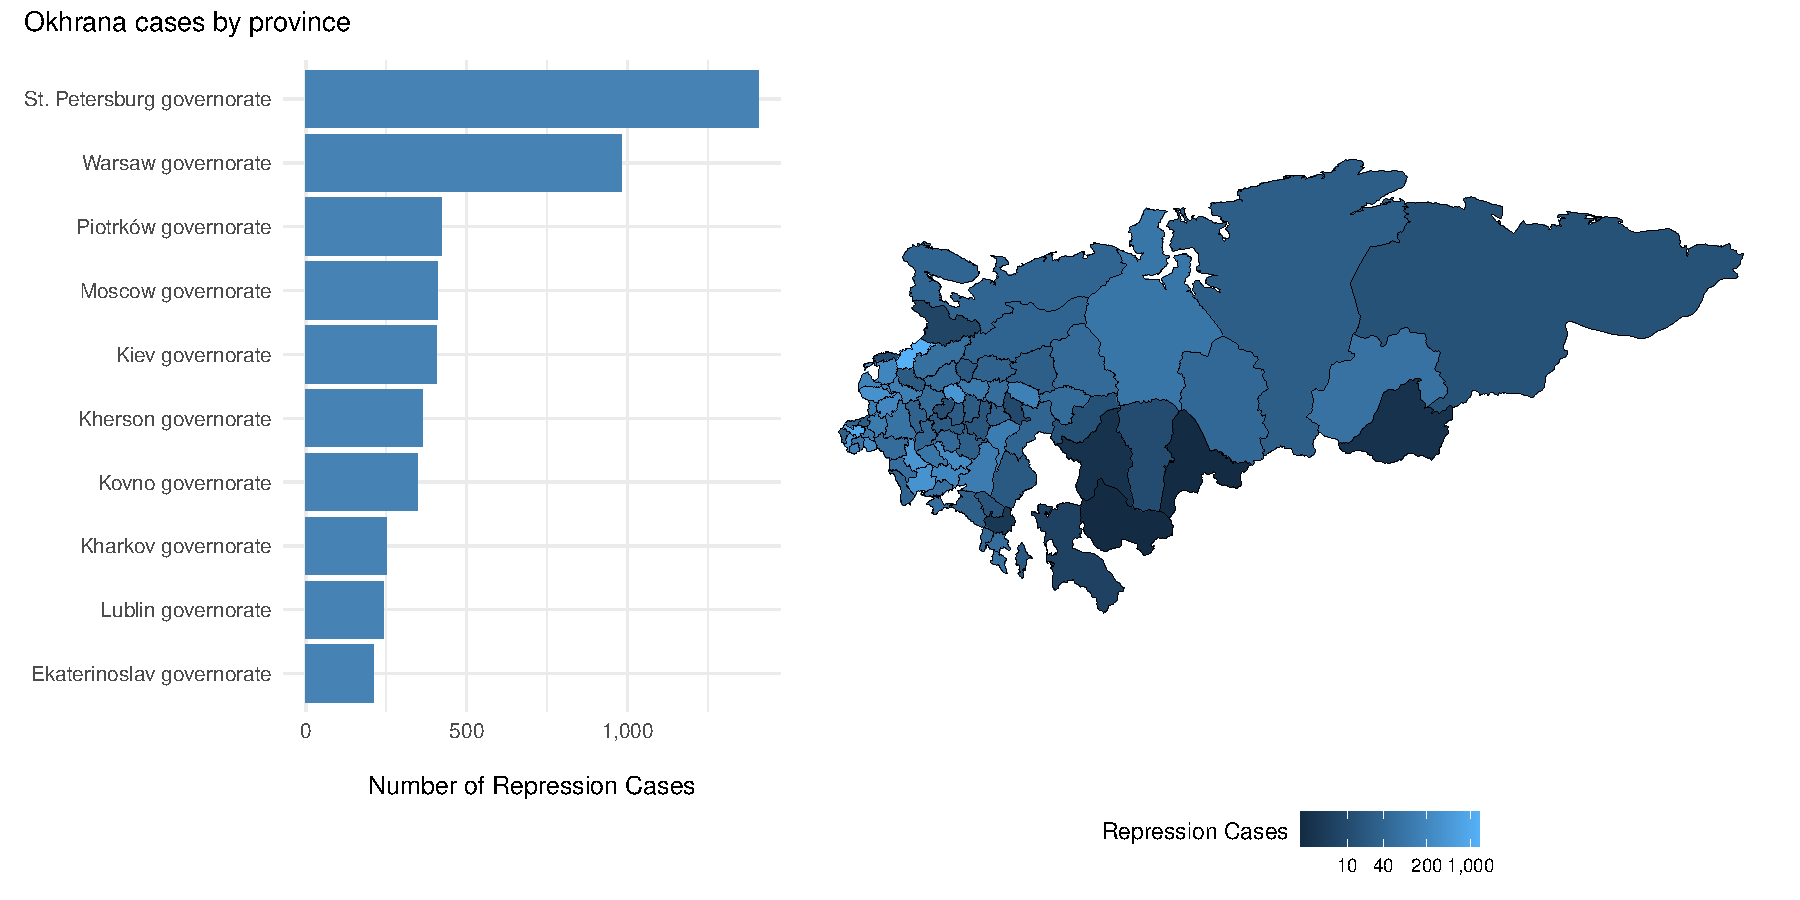
\includegraphics[keepaspectratio]{models_files/figure-pdf/descriptives-1.pdf}}

\begin{Shaded}
\begin{Highlighting}[]
\CommentTok{\# write to paper/ as okhrana\_by\_province.png}
\FunctionTok{ggsave}\NormalTok{(}\FunctionTok{here}\NormalTok{(}\StringTok{"paper"}\NormalTok{, }\StringTok{"okhrana\_by\_province.png"}\NormalTok{), }
\NormalTok{       okhrana\_by\_province, }\AttributeTok{width =} \DecValTok{12}\NormalTok{, }\AttributeTok{height =} \DecValTok{6}\NormalTok{, }\AttributeTok{dpi =} \DecValTok{300}\NormalTok{)}
\end{Highlighting}
\end{Shaded}

\begin{Shaded}
\begin{Highlighting}[]
\CommentTok{\# Refit models}
\NormalTok{model1 }\OtherTok{\textless{}{-}} \FunctionTok{lm}\NormalTok{(}\FunctionTok{log1p}\NormalTok{(total\_cases) }\SpecialCharTok{\textasciitilde{}} \FunctionTok{log1p}\NormalTok{(events), }\AttributeTok{data =}\NormalTok{ okhrana\_full)}
\NormalTok{model2 }\OtherTok{\textless{}{-}} \FunctionTok{lm}\NormalTok{(}\FunctionTok{log1p}\NormalTok{(total\_cases) }\SpecialCharTok{\textasciitilde{}} \FunctionTok{log1p}\NormalTok{(events) }\SpecialCharTok{+}\NormalTok{ land\_gini, }\AttributeTok{data =}\NormalTok{ okhrana\_full)}
\NormalTok{model3 }\OtherTok{\textless{}{-}} \FunctionTok{lm}\NormalTok{(}\FunctionTok{log1p}\NormalTok{(total\_cases) }\SpecialCharTok{\textasciitilde{}} \FunctionTok{log1p}\NormalTok{(events) }\SpecialCharTok{+}\NormalTok{ land\_gini }\SpecialCharTok{+}\NormalTok{ sh\_serfs1858 }\SpecialCharTok{+}\NormalTok{ peasant\_share, }\AttributeTok{data =}\NormalTok{ okhrana\_full)}
\NormalTok{model4 }\OtherTok{\textless{}{-}} \FunctionTok{lm}\NormalTok{(}\FunctionTok{log1p}\NormalTok{(total\_cases) }\SpecialCharTok{\textasciitilde{}} \FunctionTok{log1p}\NormalTok{(events) }\SpecialCharTok{+}\NormalTok{ land\_gini }\SpecialCharTok{+}\NormalTok{ sh\_serfs1858 }\SpecialCharTok{+}\NormalTok{ peasant\_share }\SpecialCharTok{+}
\NormalTok{               urbanization\_1904 }\SpecialCharTok{+}\NormalTok{ manufacturing\_share\_1904, }\AttributeTok{data =}\NormalTok{ okhrana\_full)}
\NormalTok{model5 }\OtherTok{\textless{}{-}} \FunctionTok{lm}\NormalTok{(}\FunctionTok{log1p}\NormalTok{(total\_cases) }\SpecialCharTok{\textasciitilde{}} \FunctionTok{log1p}\NormalTok{(events) }\SpecialCharTok{+}\NormalTok{ land\_gini }\SpecialCharTok{+}\NormalTok{ sh\_serfs1858 }\SpecialCharTok{+}\NormalTok{ peasant\_share }\SpecialCharTok{+}
\NormalTok{               urbanization\_1904 }\SpecialCharTok{*}\NormalTok{ land\_gini }\SpecialCharTok{+}\NormalTok{ manufacturing\_share\_1904, }\AttributeTok{data =}\NormalTok{ okhrana\_full)}

\CommentTok{\# Extract all term names used across models}
\NormalTok{all\_terms }\OtherTok{\textless{}{-}} \FunctionTok{unique}\NormalTok{(}\FunctionTok{unlist}\NormalTok{(}\FunctionTok{lapply}\NormalTok{(}\FunctionTok{list}\NormalTok{(model1, model2, model3, model4, model5), }\ControlFlowTok{function}\NormalTok{(m) }\FunctionTok{names}\NormalTok{(}\FunctionTok{coef}\NormalTok{(m)))))}

\CommentTok{\# Create a default mapping that falls back to original names if not mapped manually}
\NormalTok{custom\_labels }\OtherTok{\textless{}{-}} \FunctionTok{c}\NormalTok{(}
  \StringTok{"log1p(events)"} \OtherTok{=} \StringTok{"(Log) Pre{-}1905 unrest"}\NormalTok{,}
  \StringTok{"land\_gini"} \OtherTok{=} \StringTok{"Land inequality (Gini)"}\NormalTok{,}
  \StringTok{"sh\_serfs1858"} \OtherTok{=} \StringTok{"Share of serfs (1858)"}\NormalTok{,}
  \StringTok{"peasant\_share"} \OtherTok{=} \StringTok{"Peasant land share"}\NormalTok{,}
  \StringTok{"urbanization\_1904"} \OtherTok{=} \StringTok{"Urbanization (1904)"}\NormalTok{,}
  \StringTok{"manufacturing\_share\_1904"} \OtherTok{=} \StringTok{"Manufacturing share (1904)"}\NormalTok{,}
  \StringTok{"land\_gini:urbanization\_1904"} \OtherTok{=} \StringTok{"Urbanization × Inequality"}\NormalTok{,}
  \StringTok{"(Intercept)"} \OtherTok{=} \StringTok{"Intercept"}
\NormalTok{)}

\CommentTok{\# Fill in any unmapped terms to avoid errors}
\NormalTok{full\_coef\_map }\OtherTok{\textless{}{-}} \FunctionTok{setNames}\NormalTok{(}
\NormalTok{  custom\_labels[all\_terms] }\SpecialCharTok{\%||\%}\NormalTok{ all\_terms,}
\NormalTok{  all\_terms}
\NormalTok{)}

\CommentTok{\# Generate clean summary}
\FunctionTok{modelsummary}\NormalTok{(}
  \FunctionTok{list}\NormalTok{(}
    \StringTok{"1. Unrest only"} \OtherTok{=}\NormalTok{ model1,}
    \StringTok{"2. + Inequality"} \OtherTok{=}\NormalTok{ model2,}
    \StringTok{"3. + Serfdom \& Peasants"} \OtherTok{=}\NormalTok{ model3,}
    \StringTok{"4. + Urban \& Industrial"} \OtherTok{=}\NormalTok{ model4,}
    \StringTok{"5. + Urban × Inequality"} \OtherTok{=}\NormalTok{ model5}
\NormalTok{  ),}
  \AttributeTok{coef\_map =}\NormalTok{ full\_coef\_map,}
  \AttributeTok{gof\_omit =} \StringTok{"IC|Log|Adj|F|Deviance|AIC|BIC"}\NormalTok{,}
  \AttributeTok{stars =} \ConstantTok{TRUE}\NormalTok{,}
  \AttributeTok{output =} \StringTok{"kableExtra"}
\NormalTok{) }\SpecialCharTok{|\textgreater{}} 
  \FunctionTok{kable\_styling}\NormalTok{(}\AttributeTok{latex\_options =} \FunctionTok{c}\NormalTok{(}\StringTok{"scale\_down"}\NormalTok{))}
\end{Highlighting}
\end{Shaded}

\begin{table}
\centering\centering
\resizebox{\ifdim\width>\linewidth\linewidth\else\width\fi}{!}{
\begin{tabular}[t]{lccccc}
\toprule
  & 1. Unrest only & 2. + Inequality & 3. + Serfdom \& Peasants & 4. + Urban \& Industrial & 5. + Urban × Inequality\\
\midrule
Intercept & \num{2.888}*** & \num{3.104}** & \num{3.190} & \num{2.403} & \num{0.939}\\
 & (\num{0.794}) & (\num{1.113}) & (\num{2.026}) & (\num{1.596}) & (\num{1.896})\\
(Log) Pre-1905 unrest & \num{0.302} & \num{0.485}+ & \num{0.352} & \num{0.534}+ & \num{0.548}*\\
 & (\num{0.194}) & (\num{0.255}) & (\num{0.339}) & (\num{0.268}) & (\num{0.265})\\
Land inequality (Gini) &  & \num{-1.241} & \num{-1.021} & \num{-1.561} & \num{0.112}\\
 &  & (\num{1.387}) & (\num{1.998}) & (\num{1.539}) & (\num{1.938})\\
Share of serfs (1858) &  &  & \num{0.543} & \num{0.060} & \num{0.279}\\
 &  &  & (\num{0.875}) & (\num{0.687}) & (\num{0.697})\\
Peasant land share &  &  & \num{0.210} & \num{-0.234} & \num{-0.625}\\
 &  &  & (\num{1.428}) & (\num{1.110}) & (\num{1.133})\\
Urbanization (1904) &  &  &  & \num{6.297}** & \num{23.888}+\\
 &  &  &  & (\num{1.826}) & (\num{12.758})\\
Manufacturing share (1904) &  &  &  & \num{0.385} & \num{-1.325}\\
 &  &  &  & (\num{3.804}) & (\num{3.957})\\
Urbanization × Inequality &  &  &  &  & \num{-19.778}\\
 &  &  &  &  & (\num{14.200})\\
\midrule
Num.Obs. & \num{52} & \num{49} & \num{49} & \num{48} & \num{48}\\
R2 & \num{0.046} & \num{0.073} & \num{0.081} & \num{0.458} & \num{0.483}\\
RMSE & \num{1.07} & \num{1.08} & \num{1.08} & \num{0.81} & \num{0.79}\\
\bottomrule
\multicolumn{6}{l}{\rule{0pt}{1em}+ p $<$ 0.1, * p $<$ 0.05, ** p $<$ 0.01, *** p $<$ 0.001}\\
\end{tabular}}
\end{table}

\begin{Shaded}
\begin{Highlighting}[]
\NormalTok{interaction }\OtherTok{\textless{}{-}} \FunctionTok{plot\_predictions}\NormalTok{(model5, }
                 \AttributeTok{condition =} \FunctionTok{c}\NormalTok{(}\StringTok{"land\_gini"}\NormalTok{,}
                               \StringTok{"urbanization\_1904"}\NormalTok{)) }\SpecialCharTok{+}
  \FunctionTok{labs}\NormalTok{(}
    \AttributeTok{x =} \StringTok{"Land inequality (Gini)"}\NormalTok{,}
    \AttributeTok{y =} \StringTok{"Predicted (log) repression cases"}\NormalTok{,}
    \AttributeTok{color =} \StringTok{"Urbanization (1904)"}\NormalTok{,}
    \AttributeTok{fill =} \StringTok{"Urbanization (1904)"}\NormalTok{,}
\NormalTok{  ) }\SpecialCharTok{+}
  \FunctionTok{scale\_color\_viridis\_d}\NormalTok{(}\AttributeTok{option =} \StringTok{"plasma"}\NormalTok{, }\AttributeTok{direction =} \SpecialCharTok{{-}}\DecValTok{1}\NormalTok{) }\SpecialCharTok{+}
  \FunctionTok{scale\_fill\_viridis\_d}\NormalTok{(}\AttributeTok{option =} \StringTok{"plasma"}\NormalTok{, }\AttributeTok{direction =} \SpecialCharTok{{-}}\DecValTok{1}\NormalTok{) }\SpecialCharTok{+}
  \FunctionTok{theme\_minimal}\NormalTok{(}\AttributeTok{base\_size =} \DecValTok{12}\NormalTok{) }\SpecialCharTok{+}
  \FunctionTok{theme}\NormalTok{(}\AttributeTok{legend.position =} \StringTok{"bottom"}\NormalTok{)}

\NormalTok{interaction}
\end{Highlighting}
\end{Shaded}

\pandocbounded{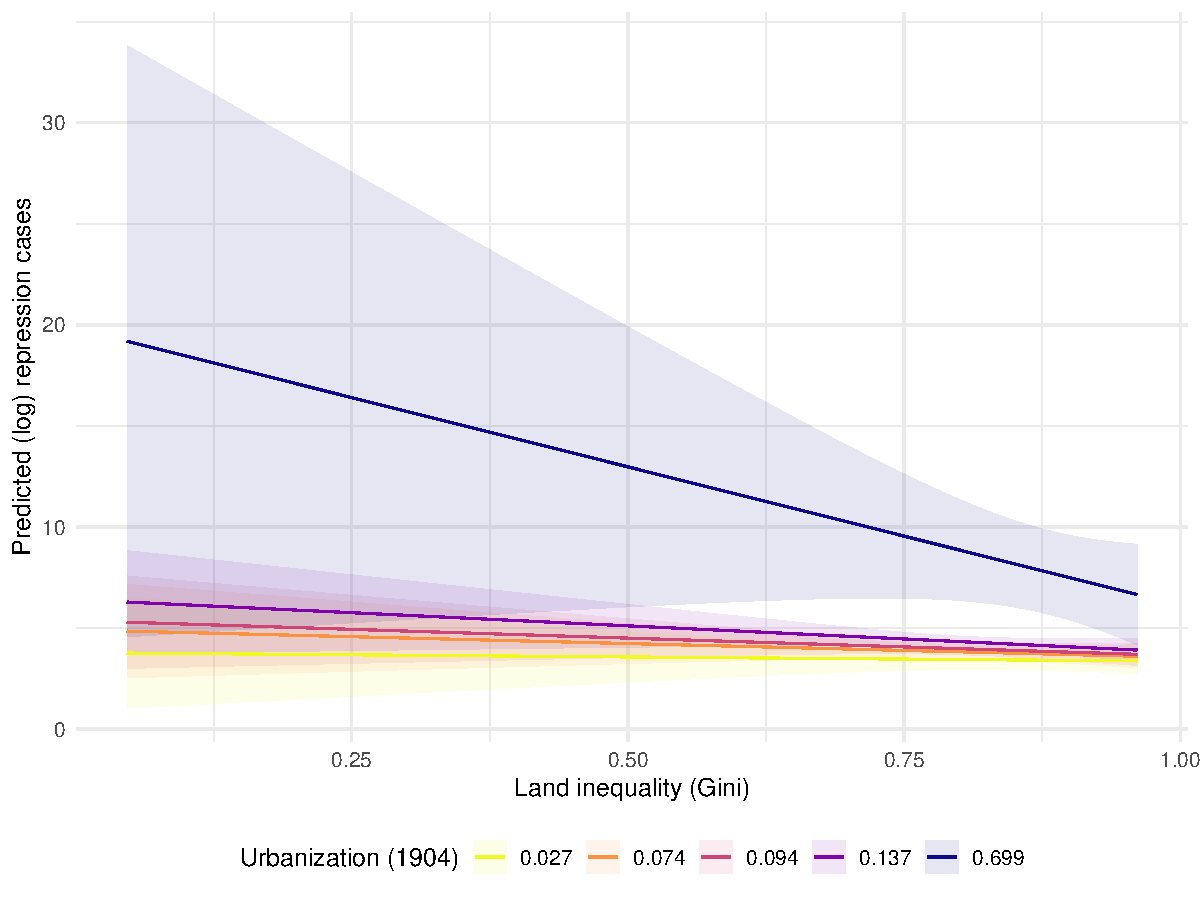
\includegraphics[keepaspectratio]{models_files/figure-pdf/plot the interaction-1.pdf}}

\begin{Shaded}
\begin{Highlighting}[]
\CommentTok{\# write to paper/ as interaction.png}
\FunctionTok{ggsave}\NormalTok{(}\FunctionTok{here}\NormalTok{(}\StringTok{"paper"}\NormalTok{, }\StringTok{"interaction.png"}\NormalTok{), }
\NormalTok{       interaction, }\AttributeTok{width =} \DecValTok{8}\NormalTok{, }\AttributeTok{height =} \DecValTok{6}\NormalTok{, }\AttributeTok{dpi =} \DecValTok{300}\NormalTok{)}
\end{Highlighting}
\end{Shaded}

\begin{Shaded}
\begin{Highlighting}[]
\NormalTok{nb\_model }\OtherTok{\textless{}{-}} \FunctionTok{glm.nb}\NormalTok{(total\_cases }\SpecialCharTok{\textasciitilde{}} \FunctionTok{log1p}\NormalTok{(events) }\SpecialCharTok{+}\NormalTok{ land\_gini }\SpecialCharTok{+}\NormalTok{ sh\_serfs1858}
                   \SpecialCharTok{+}\NormalTok{ peasant\_share }\SpecialCharTok{+}\NormalTok{ urbanization\_1904}
                   \SpecialCharTok{+}\NormalTok{ manufacturing\_share\_1904,}
                   \AttributeTok{data =}\NormalTok{ okhrana\_full)}

\NormalTok{model\_rev }\OtherTok{\textless{}{-}} \FunctionTok{lm}\NormalTok{(}\FunctionTok{log1p}\NormalTok{(revolutionary\_cases) }\SpecialCharTok{\textasciitilde{}} \FunctionTok{log1p}\NormalTok{(events) }\SpecialCharTok{+}\NormalTok{ land\_gini }
                \SpecialCharTok{+}\NormalTok{ sh\_serfs1858 }\SpecialCharTok{+}\NormalTok{ peasant\_share}
                \SpecialCharTok{+}\NormalTok{ urbanization\_1904 }\SpecialCharTok{+}\NormalTok{ manufacturing\_share\_1904, }
                \AttributeTok{data =}\NormalTok{ okhrana\_full)}

\NormalTok{model\_pop }\OtherTok{\textless{}{-}} \FunctionTok{lm}\NormalTok{(}\FunctionTok{log1p}\NormalTok{(total\_cases) }\SpecialCharTok{\textasciitilde{}}  \FunctionTok{log1p}\NormalTok{(events) }\SpecialCharTok{+}\NormalTok{ land\_gini}
                \SpecialCharTok{+}\NormalTok{ sh\_serfs1858 }\SpecialCharTok{+}\NormalTok{ peasant\_share }\SpecialCharTok{+}\NormalTok{ urbanization\_1904}
                \SpecialCharTok{+}\NormalTok{ manufacturing\_share\_1904 }\SpecialCharTok{+}
                  \FunctionTok{log}\NormalTok{(population\_1904),}
                \AttributeTok{data =}\NormalTok{ okhrana\_full)}

\NormalTok{model\_alt\_ineq }\OtherTok{\textless{}{-}} \FunctionTok{lm}\NormalTok{(}\FunctionTok{log1p}\NormalTok{(total\_cases) }\SpecialCharTok{\textasciitilde{}} \FunctionTok{log1p}\NormalTok{(events)}
                     \SpecialCharTok{+}\NormalTok{ peasant\_share }\SpecialCharTok{+}\NormalTok{ sh\_serfs1858}
                     \SpecialCharTok{+}\NormalTok{ urbanization\_1904 }\SpecialCharTok{+}\NormalTok{ manufacturing\_share\_1904,}
                    \AttributeTok{data =}\NormalTok{ okhrana\_full)}

\FunctionTok{modelsummary}\NormalTok{(}
  \FunctionTok{list}\NormalTok{(}\StringTok{"Control for population"} \OtherTok{=}\NormalTok{ model\_pop,}
       \StringTok{"Revolutionaries only"} \OtherTok{=}\NormalTok{ model\_rev,}
       \StringTok{"Alternative inequality measure"} \OtherTok{=}\NormalTok{ model\_alt\_ineq,}
       \StringTok{"Negative Binomial"} \OtherTok{=}\NormalTok{ nb\_model),}
  \AttributeTok{coef\_map =}\NormalTok{ full\_coef\_map,}
  \AttributeTok{exponentiate =} \FunctionTok{c}\NormalTok{(F, F, F, T),}
  \AttributeTok{stars =} \ConstantTok{TRUE}\NormalTok{,}
  \AttributeTok{output =} \StringTok{"kableExtra"}
\NormalTok{) }\SpecialCharTok{|\textgreater{}} 
  \FunctionTok{kable\_styling}\NormalTok{(}\AttributeTok{latex\_options =} \FunctionTok{c}\NormalTok{(}\StringTok{"scale\_down"}\NormalTok{))}
\end{Highlighting}
\end{Shaded}

\begin{table}
\centering\centering
\resizebox{\ifdim\width>\linewidth\linewidth\else\width\fi}{!}{
\begin{tabular}[t]{lcccc}
\toprule
  & Control for population & Revolutionaries only & Alternative inequality measure & Negative Binomial\\
\midrule
Intercept & \num{-9.718}* & \num{2.241} & \num{1.208} & \num{31.326}*\\
 & (\num{3.881}) & (\num{1.557}) & (\num{1.076}) & (\num{43.501})\\
(Log) Pre-1905 unrest & \num{0.154} & \num{0.661}* & \num{0.465}+ & \num{1.799}*\\
 & (\num{0.265}) & (\num{0.262}) & (\num{0.260}) & (\num{0.420})\\
Land inequality (Gini) & \num{-1.877} & \num{-2.277} &  & \num{0.082}+\\
 & (\num{1.379}) & (\num{1.502}) &  & (\num{0.109})\\
Share of serfs (1858) & \num{0.302} & \num{-0.289} & \num{0.110} & \num{1.012}\\
 & (\num{0.619}) & (\num{0.670}) & (\num{0.686}) & (\num{0.604})\\
Peasant land share & \num{0.501} & \num{-0.601} & \num{0.553} & \num{0.475}\\
 & (\num{1.017}) & (\num{1.084}) & (\num{0.794}) & (\num{0.459})\\
Urbanization (1904) & \num{5.653}** & \num{4.182}* & \num{6.286}** & \num{593.362}***\\
 & (\num{1.644}) & (\num{1.782}) & (\num{1.827}) & (\num{934.820})\\
Manufacturing share (1904) & \num{1.221} & \num{2.336} & \num{0.216} & \num{0.709}\\
 & (\num{3.411}) & (\num{3.712}) & (\num{3.802}) & (\num{2.331})\\
\midrule
Num.Obs. & \num{48} & \num{48} & \num{48} & \num{48}\\
R2 & \num{0.577} & \num{0.390} & \num{0.445} & \\
R2 Adj. & \num{0.503} & \num{0.301} & \num{0.378} & \\
AIC & \num{520.2} & \num{472.8} & \num{529.4} & \num{531.2}\\
BIC & \num{537.1} & \num{487.8} & \num{542.4} & \num{546.2}\\
Log.Lik. & \num{-51.947} & \num{-56.729} & \num{-58.502} & \num{-257.593}\\
F & \num{7.806} & \num{4.377} & \num{6.725} & \num{7.637}\\
RMSE & \num{0.71} & \num{0.79} & \num{0.82} & \num{183.58}\\
\bottomrule
\multicolumn{5}{l}{\rule{0pt}{1em}+ p $<$ 0.1, * p $<$ 0.05, ** p $<$ 0.01, *** p $<$ 0.001}\\
\end{tabular}}
\end{table}




\end{document}
